\documentclass[a4paper]{article}

\usepackage[english]{babel}
\usepackage[utf8x]{inputenc}
\usepackage[T1]{fontenc}
\usepackage[a4paper,top=3cm,bottom=2cm,left=3cm,right=3cm,marginparwidth=1.75cm]{geometry}
\usepackage{amsmath}
\usepackage{graphicx}
\usepackage[colorinlistoftodos]{todonotes}
\usepackage[colorlinks=true, allcolors=blue]{hyperref}
\usepackage{mathtools}
\usepackage{tabularx}
\usepackage{graphicx}
\usepackage{flexisym}
\usepackage{listings}
\usepackage{xcolor}
\usepackage{hyperref}
\usepackage{amsthm}
\usepackage[font={scriptsize}]{subcaption}
\title{Project 4\\ Monte Carlo simulations for Ising model}
\author{Anna Gribkovskaya}

\begin{document}
\maketitle

\begin{abstract}
In the project phase transitions in ferromagnetic material have been studied. We used the Monte Carlo method and Metropolis sampling rule to simulate the Ising model for energy and magnetization of the material. Also, periodic boundary conditions were used. We have calculated the expectation values for energy and magnetization, as well as values for heat capacity and magnetic susceptibility. The behavior near critical point has been studied and the critical temperature was obtains. All the result are in a good agreement with the solutions obtained for the closed form. The critical temperature turned to be close to the exact result obtained by Lars Onsager. 

\end{abstract}

\section*{Introduction}
The project is devoted to study of phase transitions in ferromagnetic material. In order to simulate such phenomena we use Monte Carlo methods for Markov processes with the Metropolis sampling rule. The material is approximated by a two dimensional square lattice, energy and magnetization are approximated using Ising model. We begin with a simple case ($2 \times 2$ lattice) that can be computed by hand and then proceed with the bigger lattices, different initial configurations, temperatures and number of Monte Carlo samples in order to study the model we have and to test it against existing solutions. The program for simulations is written in C++, and the Open MPI library is used for parallelization of the code.

Structure of the report:
\begin{itemize}
\item In section  \ref{Theoretical background} a brief description of the theoretical background is provided. This part is divided into few smaller ones, considering the model we are going to use and also the simplest possible examples of it's implementation.
\item In the next section \ref{Implementation} we present a description of the algorithm and some details of it's implementation in our program. Some theoretical description of Markov process and Metropolis sampling is also provided.
\item The next section \ref{RD} present all the obtained results and some analysis. It contain plots showing thermalization for the parameters together with plots for phase transitions study. 
\item In the last section \ref{Conclusion} all the obtained results are summarized and also some possibilities for further study are presented.
\end{itemize}

\section{Theoretical background} \label{Theoretical background}
\subsection{Spontaneous magnetization an phase transitions of the second order}
In this project we study phase transitions of second order taking place in a ferromagnetic material. Ferromagnet is a system with a spontaneous magnetic moment even though there is no external magnetic field around \cite{three}. This phenomena is usually explained by assuming that electron spins and magnetic moments are arranged somehow inside in a regular manner. This spontaneous magnetizations is an order parameter for ferromagnetic material under phase transitions of second order. Such phase transitions is associated with a continuous symmetry to be broken, which leads to a divergence of a second order derivative for a corresponding thermodynamical potential. From the theoretical point of view this is a challenging task to show such discontinuity, because one need to consider all possible micro-states which is hard to perform. In this project we show how it can be done by using Monte Carlo methods. However, one should make some assumptions and simplifications in order do this. 
 
\subsection{Ising Model: assumptions and simplifications}
Simplified models help us to understand the nature behind the sudden changes of properties of materials, which take place during the phase transitions. One of such models is Ising model for magnetic materials.  This is a widely used model in statistical physics. Below is a list of assumptions one should make to implement it:

\begin{itemize}
\item material under consideration is represented by a magnetic atoms, allocated in a regular lattice;
\item all atoms have magnetic moments and interact with each other thought the exchange interaction;
\item the interaction take place only between the nearest neighbors;
\end{itemize}


Using this assumptions the energy in Ising model can be presented as:

\begin{equation}
E=-J\sum_{\langle kl\rangle }^{N}s_{k}s_{l} -B\sum_{k}^{N}s_{k} 
\end{equation}
here $N$ is total number of spins, $J$ is a coupling constant that express the
strength of interaction between spins, $B$ represent external magnetic field and symbol $s_{k}=\pm 1$, $\langle kl\rangle $ represent the sum over neighboring spins only.

The second term in this formula stands for external magnetic field, which is zero for simplicity. Another simplification is interaction between neighboring spins only. In general it is not a problem to study a long-range interactions between spins in the lattice and include an external magnetic field in the model, however this will turn our project into a thesis. One more simplification is the structure under consideration. We consider square lattice in $x$ and $y$ directions. There are many other types of structures available. For instance one may use triangles or extend the lattice to three dimensions. Those who are interested can refer to \cite{one}. \\
With a square lattice of a finite size we have to be a bit careful when it comes to the boundary. There are two most popular approaches to deal with spins on the boundaries: the free-ends and the periodic boundary conditions (PBC). In this project we implement the PBC. It means, that for every spin on the boundary we assume to interact with the "virtual" spin on the other boundary. For example, in the first row the spin on the right boundary interact with the first spin and in the first column the bottom spin interact with the first one. 

\subsection{Thermodynamics and Statistical physics}
As soon as we are going to study the phase transitions in the ferromagnetic material, we need to choose ensemble which consider temperature as an intensive variable and it is surely the Canonical Ensemble. In this case the probability distribution is given by Boltzmann distribution and the potential is Helmholtz free energy. Some formulas we may need in the calculations:

\begin{equation}
P_{i}(\beta) =\frac{e^{-\beta E_{i}}}{Z} \\
\end{equation}

with $\beta = 1/k_{B}T$ being the inverse temperature, $k_{B}$ is the Boltzmann constant, $E_{i}$ is the energy of a micro-state $i$. The partition function Z is given by:
\begin{equation}
Z=\sum_{i=1}^{M}e^{-\beta E_{i}}
\end{equation}
here M sum over all micro-states. 
Expressions for the mean values of energy and magnetization will be given as follows:
\begin{eqnarray}
\langle E\rangle &=&\frac{1}{Z}\sum_{i}^{M}E_{i}e^{-\beta E_{i}} \\
\langle M\rangle &=&\frac{1}{Z}\sum_{i}^{M}M_{i}e^{-\beta E_{i}}
\end{eqnarray}
here $M_{i}$ magnetization for microstate $i$, 
The number of microstates in our case (quadratic lattice in 2D) can be obtained
as $2^{L\times L}$, with $L$ representing the lattice size.

\subsubsection{Example for 2 by 2 lattice}
The Ising model provide us with an easy way to calculate the energy of a single micro-state. However, even for the case in two dimensions and a quadratic lattice the number of spins increase as ${L\times L}$, with $L$ representing the lattice size. The total number of micro-states will be then $2^{L\times L}$. The simplest case of a quadratic lattice is the case for $2\times 2$ lattice and for such lattice it is possible (but of course a bit boring) to calculate partition function and all other values, such as heat capacity and susceptibility (as they can be expressed in a form of second order derivatives of the partition function). 


For $2\times 2$ lattice we would have just 16 micro-states and that allow us to calculate all needed parameters for all possible micro-states by hand. Below is what we get.

\begin{table}[h!]
  \caption{Values of energy and magnetization for two-dimensional Ising model of magnetic with square lattice. Lattice size is 2$\times$2. Periodic boundary conditions were used.}
  \label{tab:2x2}
  \begin{center}
    \begin{tabular}{c|c|c|c}
    \hline
		Number of spins up & Degeneracy & Energy, $J$ & Magnetization, M \\
        \hline
	$	0 $  & $ 1 $ & $ -8 $ & $ -4 $  \\
	$	1 $  & $ 4 $ & $  0 $ & $ -2 $  \\
	$	2 $  & $ 2 $ & $  8 $ & $ 0  $  \\
	$	2 $  & $ 4 $ & $  0 $ & $ 0  $  \\
	$	3 $  & $ 4 $ & $  0 $ & $ 2  $  \\
  $	4 $  & $ 1 $ & $  8 $ & $ 4  $  \\

	\end{tabular}
  \end{center}
\end{table}

 The closed form expression for the partition function is:

\begin{equation}
z=\sum_{i}^{M}e^{-\beta E_{i}}=\sum_{E}\Omega (E)e^{-\beta E}
\end{equation}

here $M$ is number of all micro-states,  $\sum_{E}$ is sum for all allowed energies, $\Omega (E)$ is degeneracy
for each energy (the number of configurations with this particular energy). 

Using the results in the table \ref{tab:2x2} above we get:
\begin{equation}
z=2e^{-8\beta J}+2e^{8\beta J}+12=4\cosh (8\beta J)+12
\end{equation}

Using (4) and (6) the expectation value for the energy can by calculated as follows:

\begin{equation*}
\langle E\rangle =\frac{1}{z}\sum_{i}^{M}E_{i}e^{-\beta E_{i}}=-\frac{
\partial \ln z}{\partial \beta }=-\frac{\partial \ln (4\cosh (8\beta J)+12)}{
\partial \beta}
\end{equation*}

Taking the derivative we get:

\begin{equation}
\langle E\rangle =-8J\frac{\sinh 8J\beta }{\cosh 8J\beta+3}
\end{equation}

Using (5) and (6) the expectation value for the absolute magnetization can by calculated as follows:

\begin{equation*}
\langle \left\vert M\right\vert \rangle =\frac{1}{z}\sum_{i}^{M}\left\vert
M_{i}\right\vert e^{-\beta E_{i}}=\frac{4e^{8\beta J}+8+8+4e^{8\beta J}}{z}
\end{equation*}

Which result in:
\begin{equation}
\langle \left\vert M\right\vert \rangle = \frac{2(e^{8\beta J}+2)}{\cosh (8\beta J)+3}
\end{equation}

With a known partition function one can also compute heat capacity and magnetic susceptibility. They are obtained as follows:

\begin{eqnarray}
C_{v} &=&\frac{\sigma^2 _{E}}{k_{B}T^{2}} \\
\chi &=&\frac{\sigma^2 _{M}}{k_{B}T}
\end{eqnarray}
here $\sigma _{E}$ is standard deviation for the energy, and $\sigma _{M}$ is is standard deviation for the magnetization.
Applying this we get:

\begin{eqnarray}
C_{v} &=&128J^{2}\frac{1+3\cosh 8J\beta }{6\sinh 8J\beta +\sinh 16J\beta }\\
\chi &=&\frac{8\beta (e^{8J\beta }+1)}{\cosh 8J\beta +3}-\left( \frac{2(e^{8\beta J}+2)}{\cosh (8\beta J)+3}\right) ^{2}
\end{eqnarray}
Using the derived formulas one can compute the values for all interesting parameters for the 2$\times$2 case. In our project we use $J=1$ and measure temperature in in $k_BT/J$ units.

\clearpage
\section{Implementation: Monte Carlo simulations, Markov chains and Metropolis sampling rule}\label{Implementation}
In this project we implement a Monte Carlo simulations based on Markov process. The reason to do so is that when Markov process run for quite a long time, it will end up in the equilibrium state, independently from the starting point. It is so, because the Markov process assume that every new move is made considering only the previous state, but not the history of all other moves. The only thing that is missing here is sampling rule. We need a rule to accept or decline a new move. In our project this is taken care of by the Metropolis sampling. Below is the algorithm we implement \cite{two}. 

\begin{enumerate}
\item
Create a ferromagnet with a random or ordered spin structure. All parameters, such as lattice size, temperature number of Monte Carlo cycles and ordered/chaotic orientation of spins are given from the command line.
\item
Calculate the energy of the initial state, using periodic boundary conditions. Also at this stage the exponents for each energy difference ($\Delta E$) are calculated ($\omega= exp(-\Delta E)$).
\item
Here the Monte Carlo (MC) simulations begin. \\
\begin{enumerate}
\item Pick up a random spin, flip it and compute the energy difference with the previous state. 
\item 
If $\Delta E < 0$ accept the new state, the spin remains flipped. 
\item 
If $\Delta E > 0$, start the Metropolis sampling. Call random number generator and compute a random number $r$ and compare it with the corresponding precalculated exponent for this specific energy difference.
\begin{enumerate}
\item if $r \leq \omega$ accept the new state, the spin remains flipped.
\item else keep the old state, flip spin back.
\end{enumerate}
\item Go back to the a). Each MC sample contain ${L\times L}$ iterations, so every spin has a chance to flip.
\end{enumerate}
\item Here we update all expectation values: energy, magnetization, absolute magnetization, energy and magnetization squared.
\end{enumerate}

It is also possible to improve our program by parallelizing code with OpenMPI library \cite{four}.  In order to implement this we divide the numerical experiment into several parallel experiments (eight in our case). After all of them are done we just need to sum up all the data and calculate the mean. This allow us to increase the speed of the program, which is very important in case of large lattices.
The source code for the program can be found on \url{https://github.com/andrei-fys/fys4150/tree/master/Project_4}. Program was written in collaboration with Andrei Kukharenka.

\clearpage
\section {Results and discussion}\label{RD}
\begin{table}[h!]
  \caption{Values of energy, magnetization, heat capacity and magnetic susceptibility for $2\times 2$ square lattice computed using Ising model and periodic boundary conditions. Temperature $1K$ and $J=1$ }
  \label{tab:2x2_compare}
  \begin{center}
    \begin{tabular}{c|c|c|c|c|c}
    \hline
        MC samples & $\langle E\rangle$ & $\langle \left\vert M\right\vert \rangle$ & $C_{v}$ & $\chi$ & relative error for $\chi$ ($\%$) \\
        \hline
    $    Exact $ & $-7.9839$ & $ 3.9946 $ & $ 0.12859 $ & $ 0.016043 $ & - \\
    $    10^5 $  & $-7.982$ & $ 3.9939 $ & $ 0.144956 $ & $ 0.0186428 $ & 16,2 \\
    $    10^6 $  & $-7.98405$ & $ 3.99465 $ & $ 0.127362 $ & $ 0.0161074 $ & 0,4 \\
    $    10^7 $  & $-7.9839$ & $ 3.99464 $ & $ 0.12856 $ & $ 0.0160516 $ & 0,05 \\

    \end{tabular}
  \end{center}
\label{table: one}  
\end{table}
Table \ref{table: one} present the results for various parameters, such as energy, magnetization, heat capacity and magnetic susceptibility for $2\times 2$ square lattice. As we can see the values are in a good agreement with the closed form solution. The most "sensitive" parameter is the magnetic susceptibility $\chi$, which needs more then $10^5$ MC samples to get close to the exact solution. When the number of MC samples increase the relative error for $\chi$ goes down quite fast. For the $10^7$ MC samples we get almost exact result from our computations. However, this is applicable only for a small lattice sizes. Even the $10^6$ MC samples are hard to perform on a lattice larger then $100 \times 100$. 
The reason why magnetic susceptibility is so sensitive to the number of MC samples can be explained by the fact it depend on fluctuations of magnetization, that has twice as small range as the energy (and only two possible $\Delta M$, while for $\Delta E$ we have five possible values). \\
Figure \ref{fig1} present the results for mean energy and mean magnetization in case of lattice $20 \times 20$ and $10^5$ MC samples. Every parameter was studied for two temperatures (T=1 and T=2.4) and two initial configurations: ordered and random. This simulations were performed to simulate the development over "time". Time in this case is represented by the number of MC samples. Thermalization here is number of MC samples needed to reach the most likely state. As one can see this number depend on the temperature (which is quite obvious) and the initial configuration. The ordered initial configuration require less MC samples to get to the equilibrium as well as lower temperature. Also, one can see that energy reach the equilibrium much faster then magnetization for both temperatures. The reason here may be the same as discussed above for the magnetic susceptibility. However this difference become less with increase of the temperature. Same is the difference for the ordered and random initial states. For larger temperatures frequency of fluctuations increase and this neutralize the effect. We perform this study to understand how many MC samples needed to reach the equilibrium, so we can use this in a future experiments and just run the simulation without recording the data, just to update the lattice configuration and start the records from the most likely state. The number of MC samples needed before we reach the equilibrium vary for different temperatures and initial configurations, but we may took approximately $15 \%$ and be on a safe ground for any of them.



\begin{figure}[h!] 
  \begin{subfigure}[b]{0.5\linewidth}
    \centering
    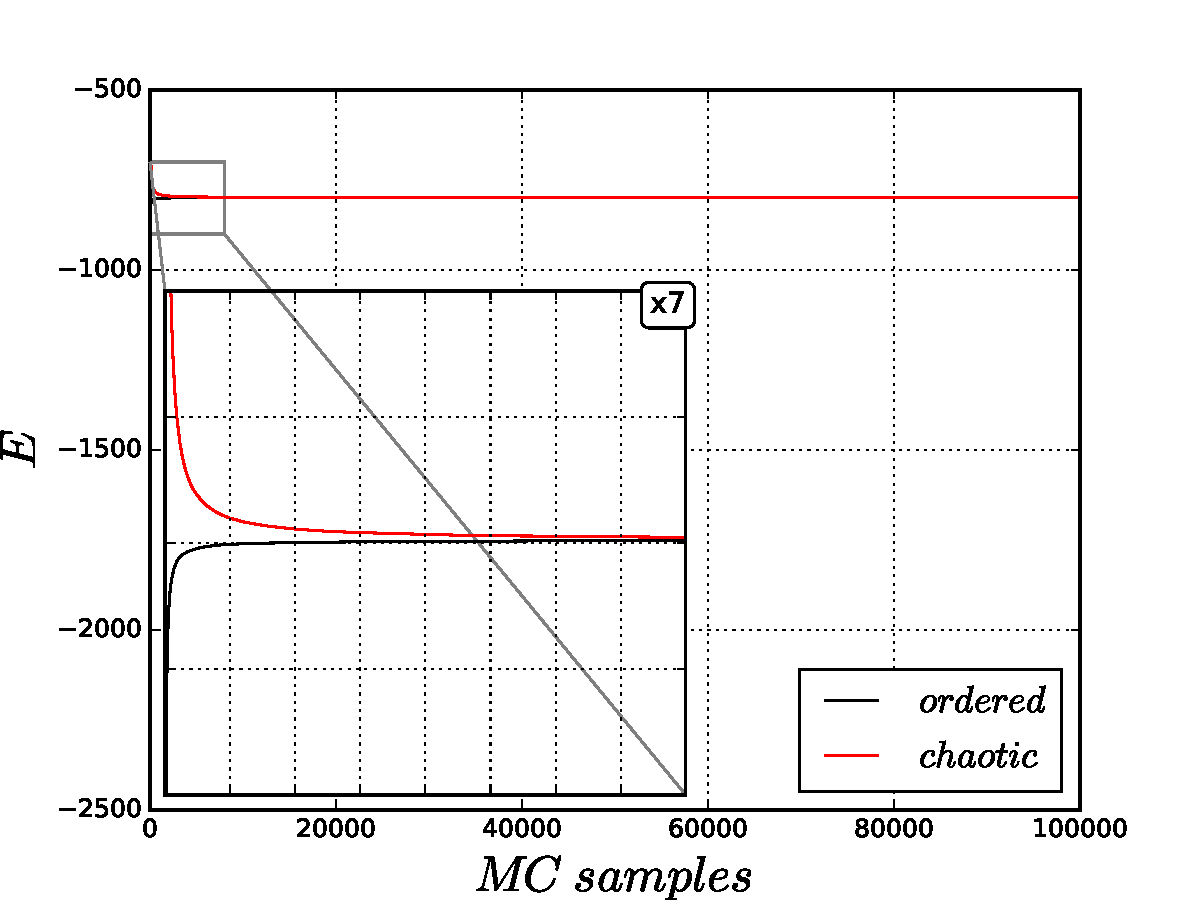
\includegraphics[width=1.0\linewidth]{20x20_10_5_1_energy} 
    \caption{Energy thermalization. \\ Lattice $20 \times 20$, MC samples is $10^5$, T=1 (in $k_BT/J$ units)} 
    \label{fig1:a} 
    \vspace{1ex}
  \end{subfigure}
  \begin{subfigure}[b]{0.5\linewidth}
    \centering
    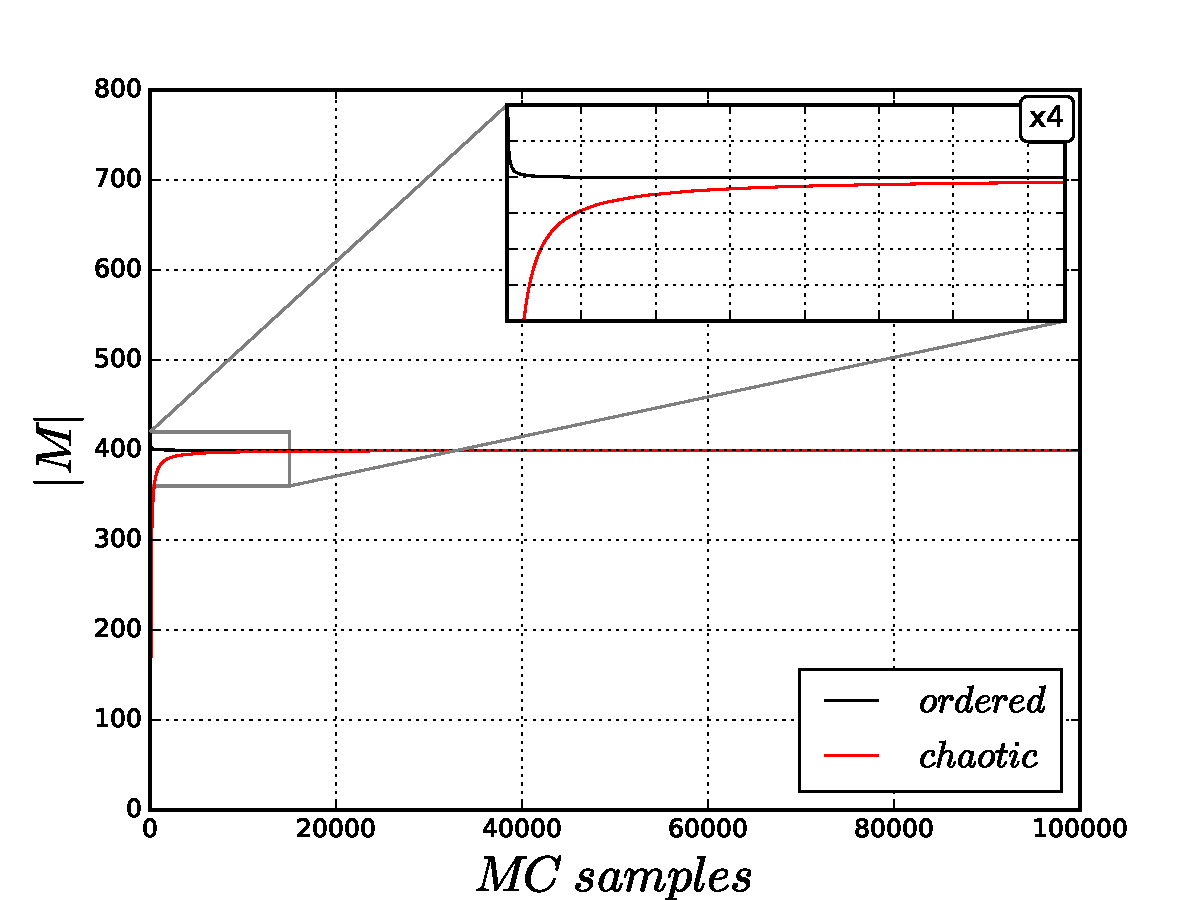
\includegraphics[width=1.0\linewidth]{20x20_10_5_1_magnet} 
    \caption{Magnetization thermalization. \\ Lattice $20 \times 20$, MC samples is $10^5$, T=1 (in $k_BT/J$ units)} 
    \label{fig1:b} 
    \vspace{1ex}
  \end{subfigure} 
  \begin{subfigure}[b]{0.5\linewidth}
    \centering
    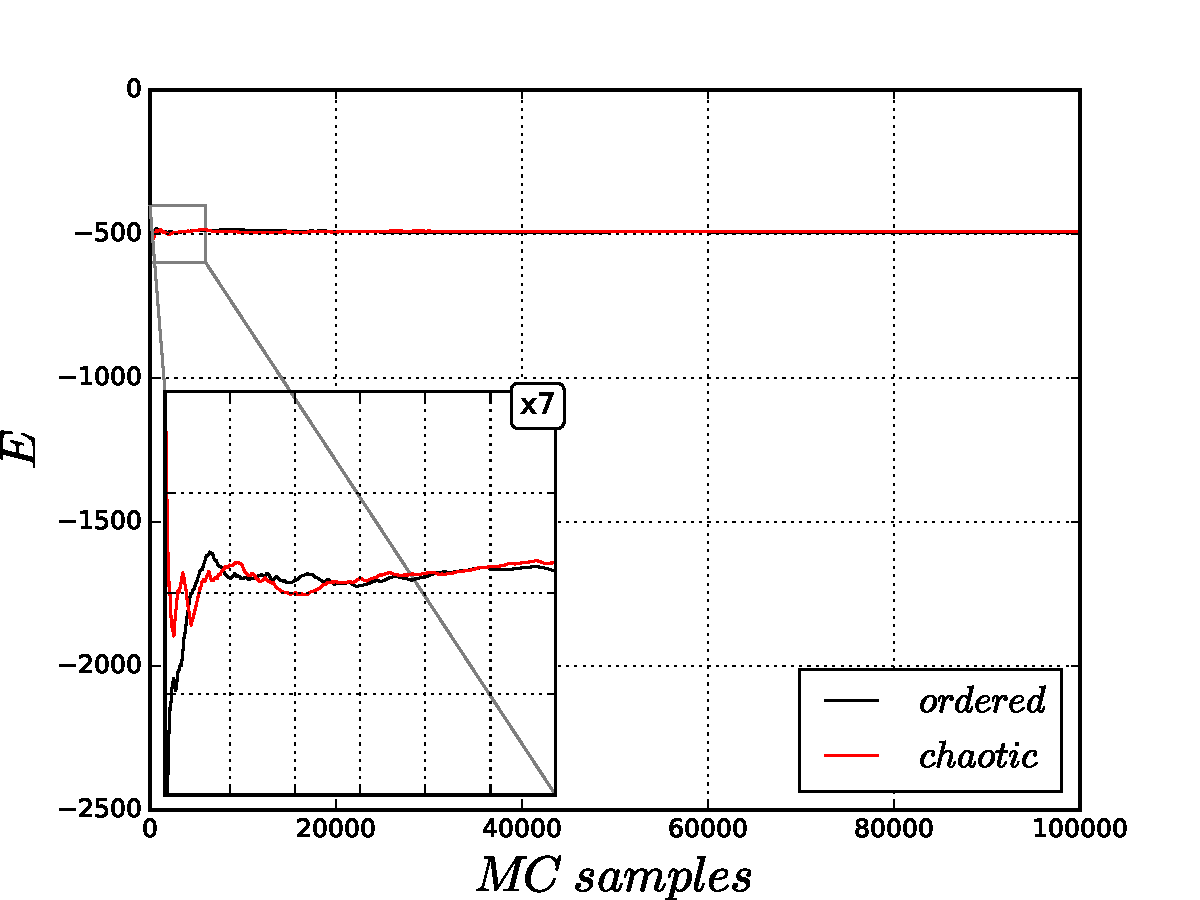
\includegraphics[width=1.0\linewidth]{20x20_10_5_24_energy} 
    \caption{Energy thermalization. \\ Lattice $20 \times 20$, MC samples is $10^5$, T=2.4 (in $k_BT/J$ units)} 
    \label{fig1:c} 
  \end{subfigure}
  \begin{subfigure}[b]{0.5\linewidth}
    \centering
    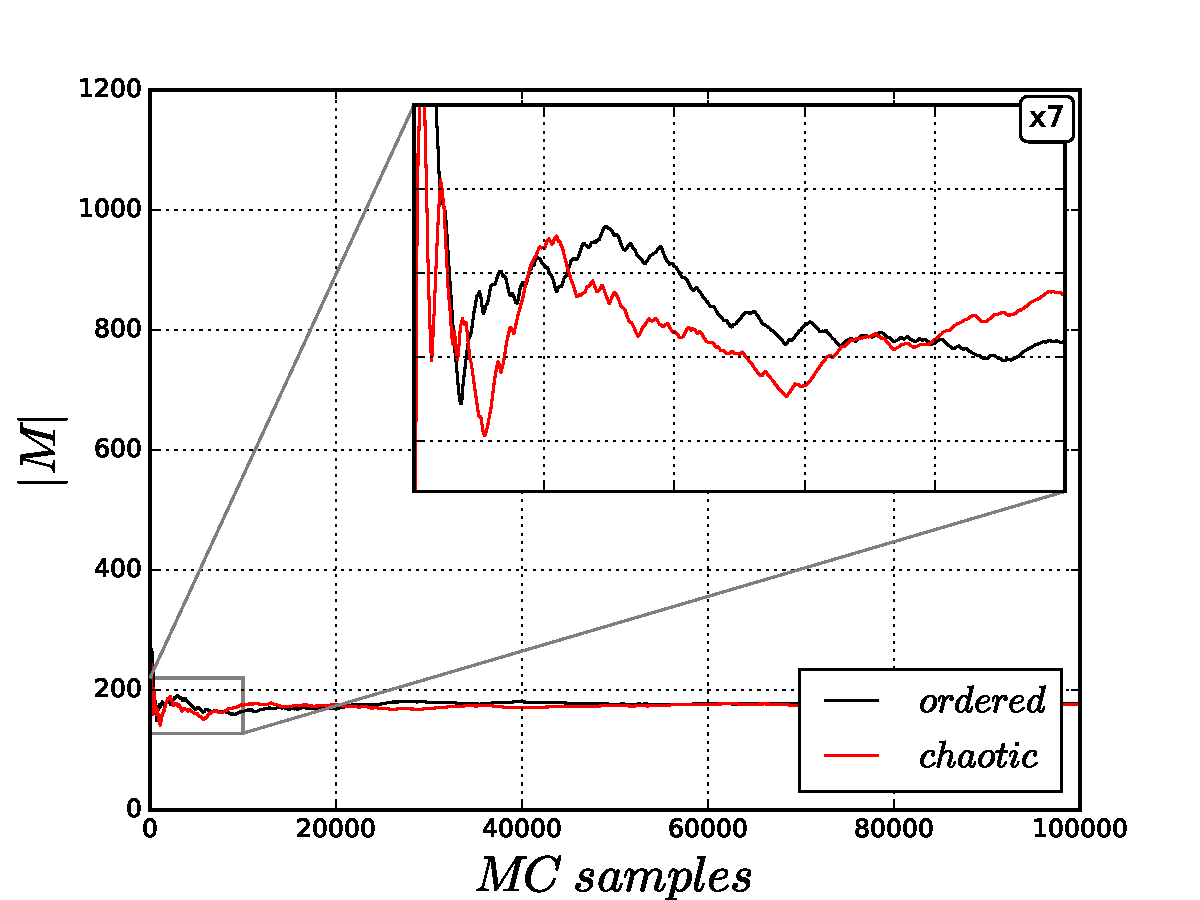
\includegraphics[width=1.0\linewidth]{20x20_10_5_24_magnet} 
    \caption{Magnetization thermalization. \\ Lattice $20 \times 20$, MC samples is $10^5$, T=1 (in $k_BT/J$ units)} 
    \label{fig1:d} 
  \end{subfigure} 
  \caption{ Energy and magnetization development over time for different temperatures. Time is represented by number of MC samples, the lattice size is $20 \times 20$, total number of MC samples is $10^5$, temperature is measured in $k_BT/J$ units }
  \label{fig1} 
\end{figure}

Figure \ref{fig2} presents the probability distributions functions (PDF) for two temperatures $T=1$ and $T=2.4$. As one can see in case of large temperature we obtain the the PDF of a Gaussian shape, with a mean value corresponding to the expectation value of the energy. For the case of smaller temperature, the number of possible energies decrease dramatically. The gap between the most probable state and second most probable state can be explained considering the orientation of spins needed for such configuration. The most likely state here is the most ordered state, with all spins pointing up or down. In general we have five possible $\Delta E$, but for this particular state the only possible move is $\Delta E =8$, because all spins have the same orientation and we are allowed to flip only one spin at the time (one may argue that the gap should be fulfilled by the moves from other configurations, but this is almost never happen as number of possible energies is very small for such temperature).

Figure \ref{fig3} presents plots we made to study the temperature development for energy, magnetization, heat capacity and magnetic susceptibility near the critical temperature. All calculations were made for different lattice sizes, so one can see the finite lattice size effect. Here we suppose to see a sign of phase transition. In theory, for the infinite lattice we should see a discontinuity in a second derivative of the thermodynamic potential in case of the second order phase transition. In our case this represented by heat capacity and magnetic susceptibility. Also, such phase transition vanishes the spontaneous magnetization of the material, so the magnetization should drop to zero.  For the finite lattice size we do not have zero magnetization, but we may see from plot \ref{fig3:c} that the larger the lattice is the smaller is the magnetization for higher temperatures. The critical temperature in our case supposed to be equal to 2.269 (in $k_BT/J$ units). 
In order to explain the finite size influence on the values for the critical temperature we are using the following scaling relation:
\begin{equation}
 T_C(L)-T_C(L=\infty) = aL^{-1/\nu},
 \label{eq:tc}
\end{equation}
here $\nu =1$, $T_C(L)$ is critical temperature obtained for the lattice size $L$ and $T_C(L=\infty)$ is the critical temperature for the infinite lattice. \\
We need to compute the value of $a$:
\begin{equation}
a=(T_C(L_1)-T_C(L_2))\frac{L_1 L_2}{L_2-L_2}
\end{equation}
In our case we have $T_C(L_1 =100)=2,29$ and $T_C(L_2 =140)=2,28$. The parameter $a=3.5$. The critical temperature in the thermodynamical limit cam be computes as:
\begin{equation}
T_C(L=\infty) = T_C(L)-\frac{3.5}{L}
\end{equation}
For the $L=140$ it is $T_C(L=\infty)= 2.255$ (in $k_BT/J$ units. Wich is quite close to the exact result after Lars Onsager, relative error is $\approx 0,6\%$.



\begin{figure}[t!] 
  \begin{subfigure}[t]{0.5\linewidth}
    \centering
    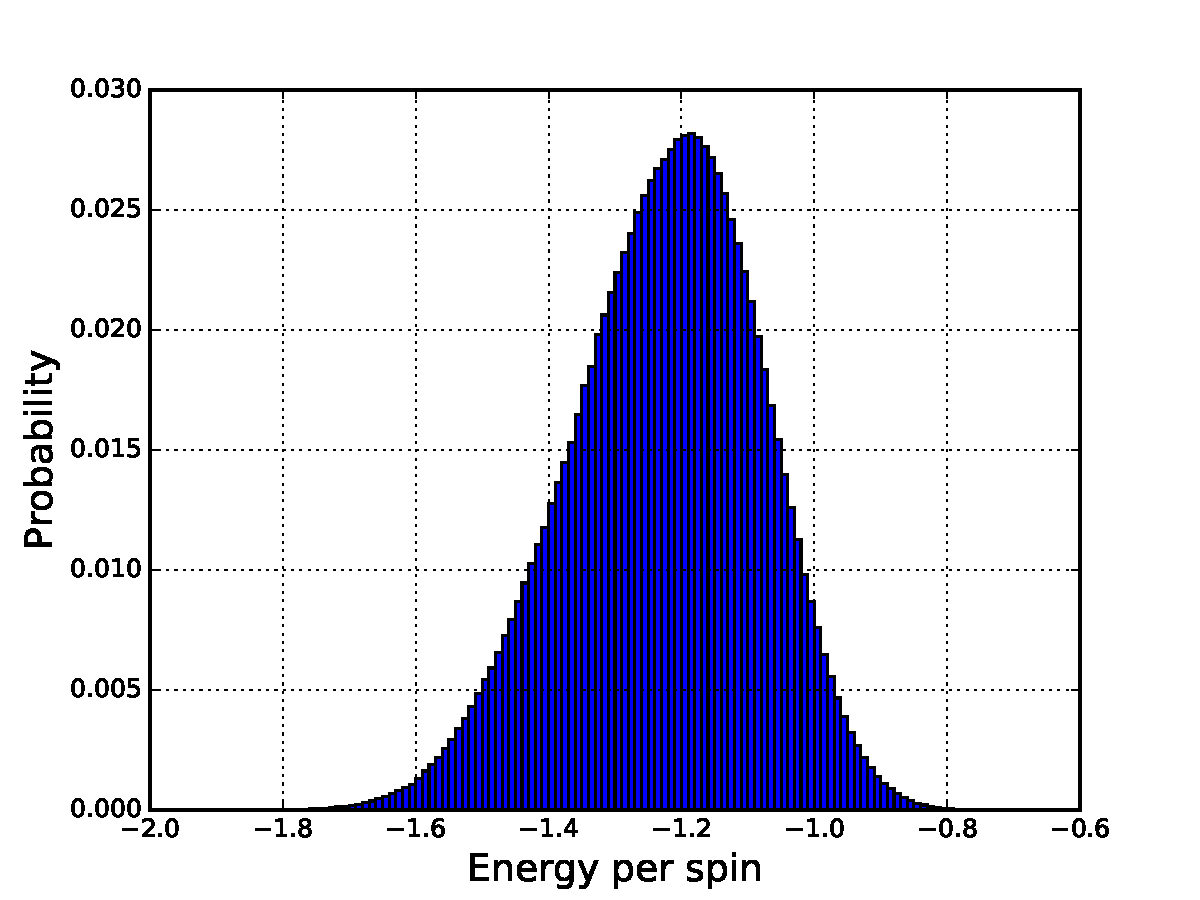
\includegraphics[width=1.0\linewidth]{Energy_pdf_20_24} 
    \caption{Temperature is 2.4} 
    \label{fig2:a} 
  \end{subfigure}
  \begin{subfigure}[t]{0.5\linewidth}
    \centering
    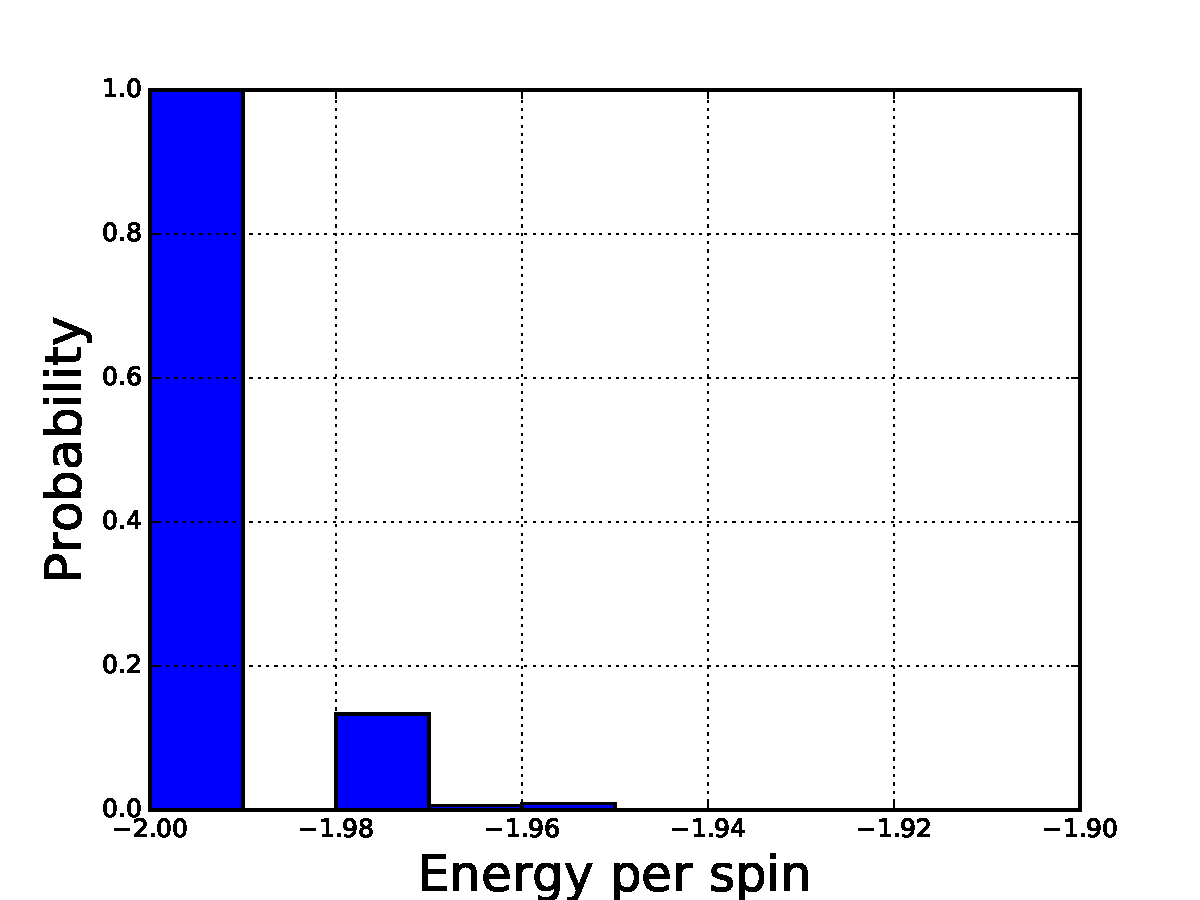
\includegraphics[width=1.0\linewidth]{Energy_pdf_20_T_1} 
    \caption{Temperature is 1} 
    \label{fig2:b} 
  \end{subfigure} 
  \caption{ Probability distribution for the energy of micro-states for system of 20$\times$20 spins. Temperature is in units of $k_BT/J$. Number of MC samples $10^5$. Energy is normalized per spin.Probability is normalized so the total probability is equal to one.   }
  \label{fig2} 
\end{figure}

\begin{figure}[h!] 
  \begin{subfigure}[b]{0.5\linewidth}
    \centering
    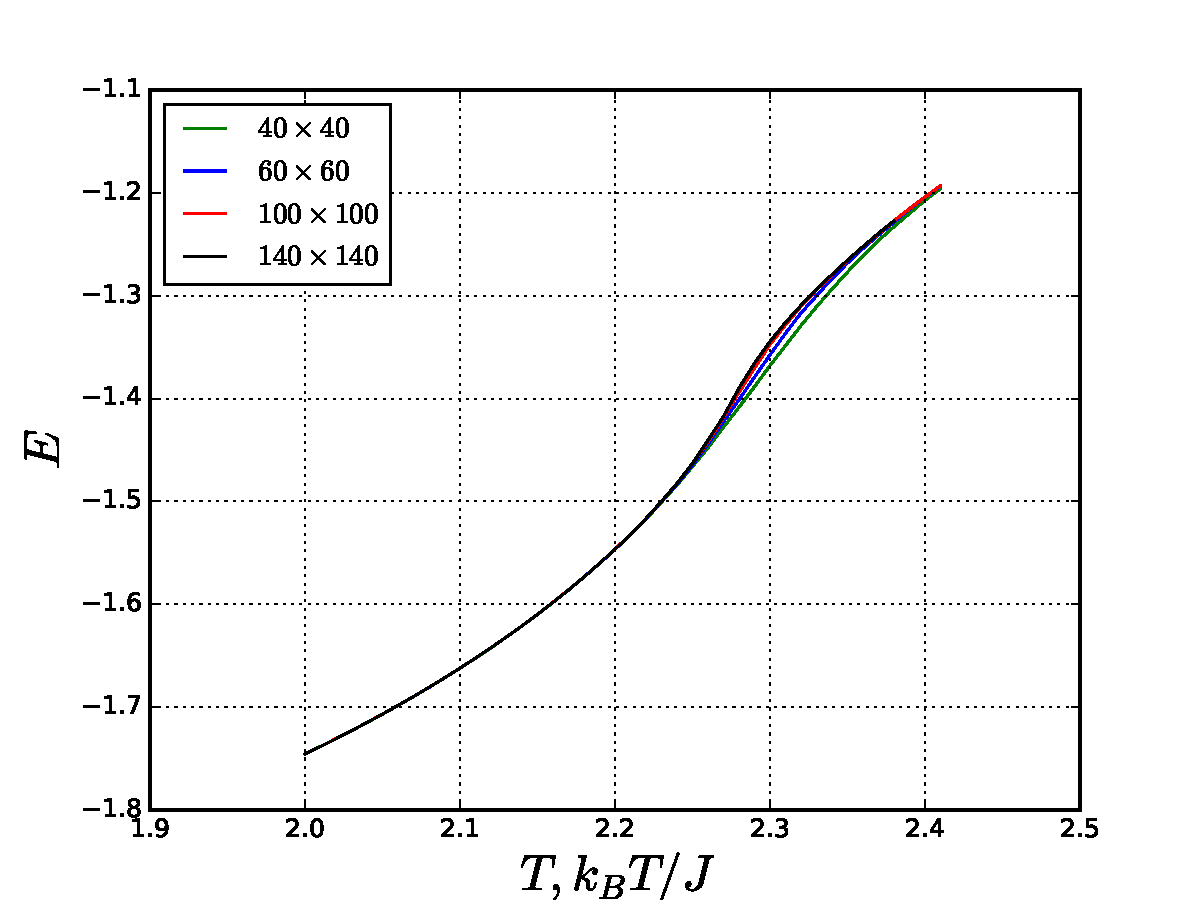
\includegraphics[width=1.0\linewidth]{phase_10_6_energy} 
    \caption{Energy development over varying temperature } 
    \label{fig3:a} 
    \vspace{1ex}
  \end{subfigure}
  \begin{subfigure}[b]{0.5\linewidth}
    \centering
    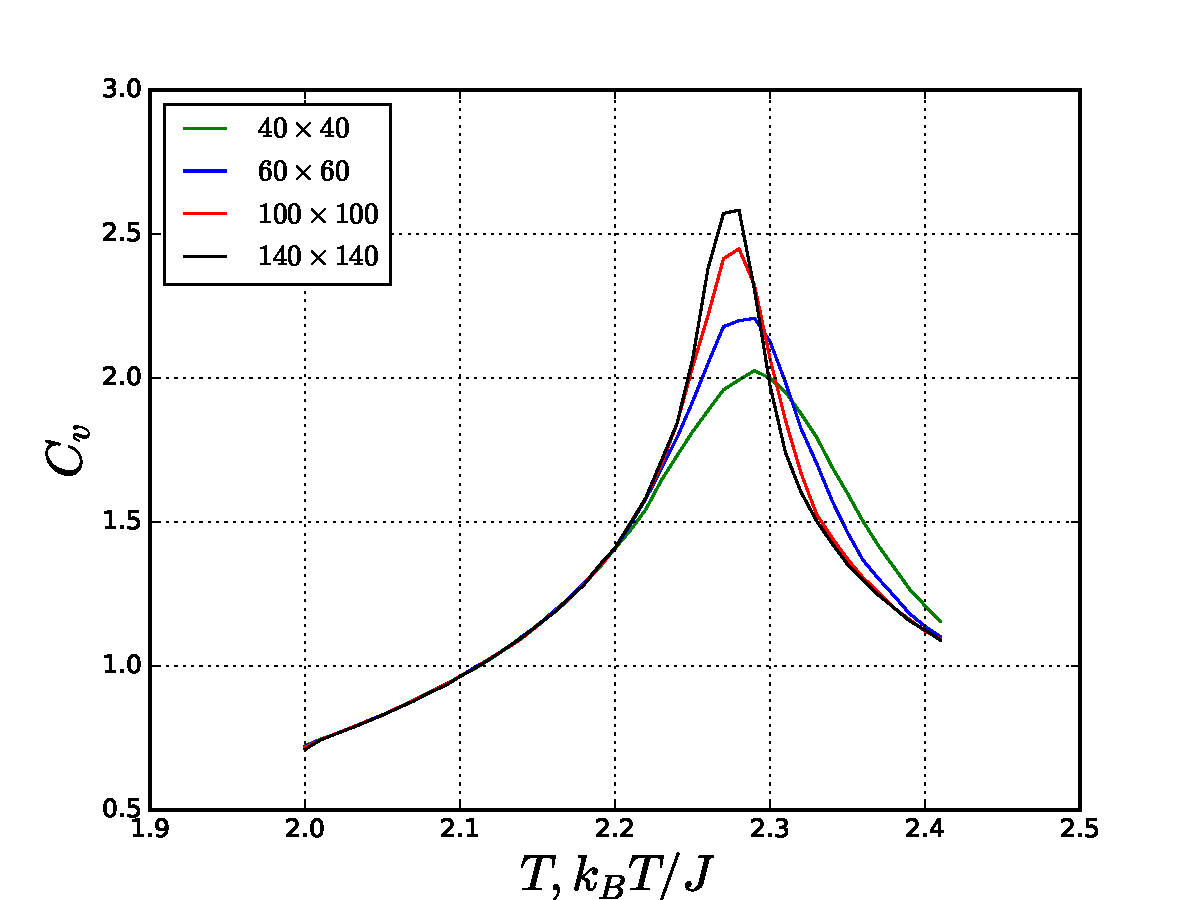
\includegraphics[width=1.0\linewidth]{phase_10_6_heat_capacity} 
    \caption{Heat capacity development over varying temperature } 
    \label{fig3:b} 
    \vspace{1ex}
  \end{subfigure} 
  \begin{subfigure}[b]{0.5\linewidth}
    \centering
    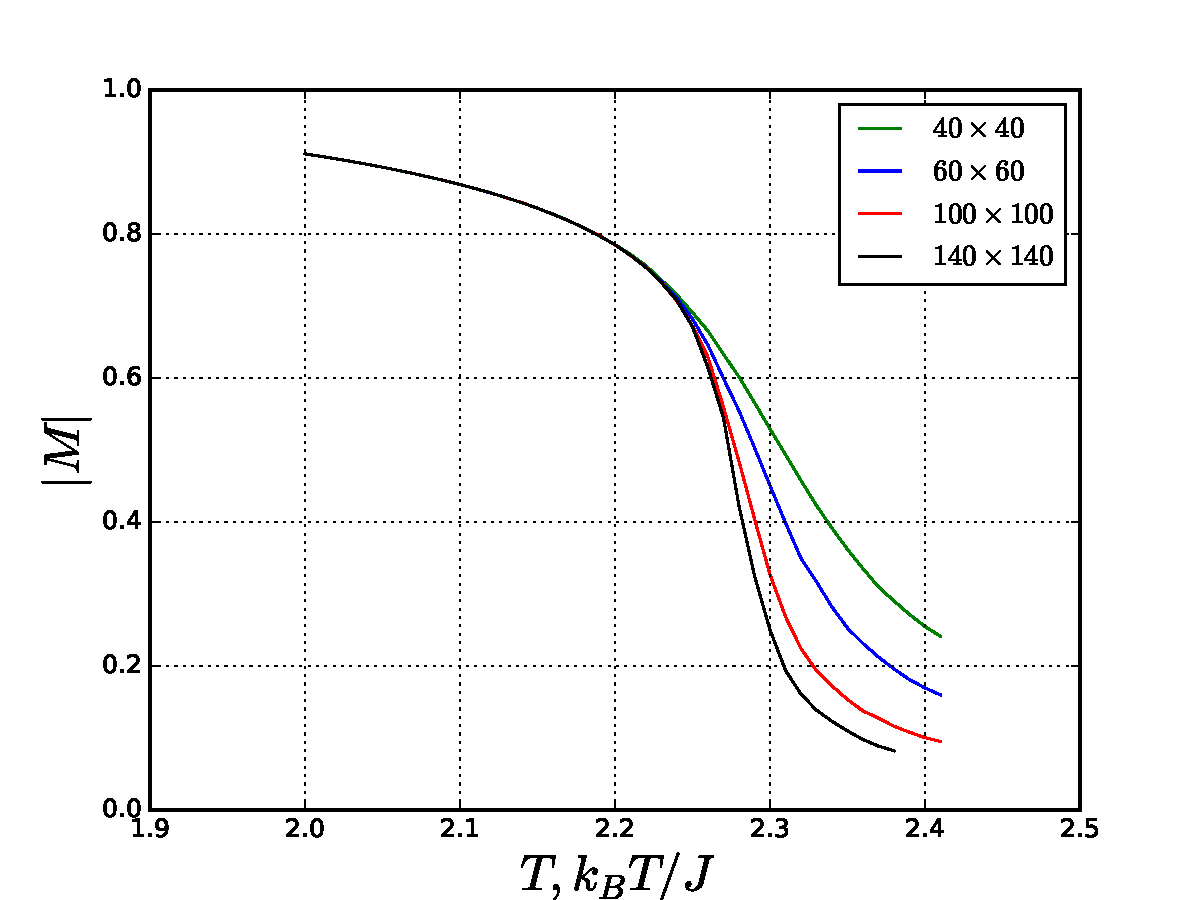
\includegraphics[width=1.0\linewidth]{phase_10_6_magnetization} 
    \caption{Magnetization development over varying temperature } 
    \label{fig3:c} 
  \end{subfigure}
  \begin{subfigure}[b]{0.5\linewidth}
    \centering
    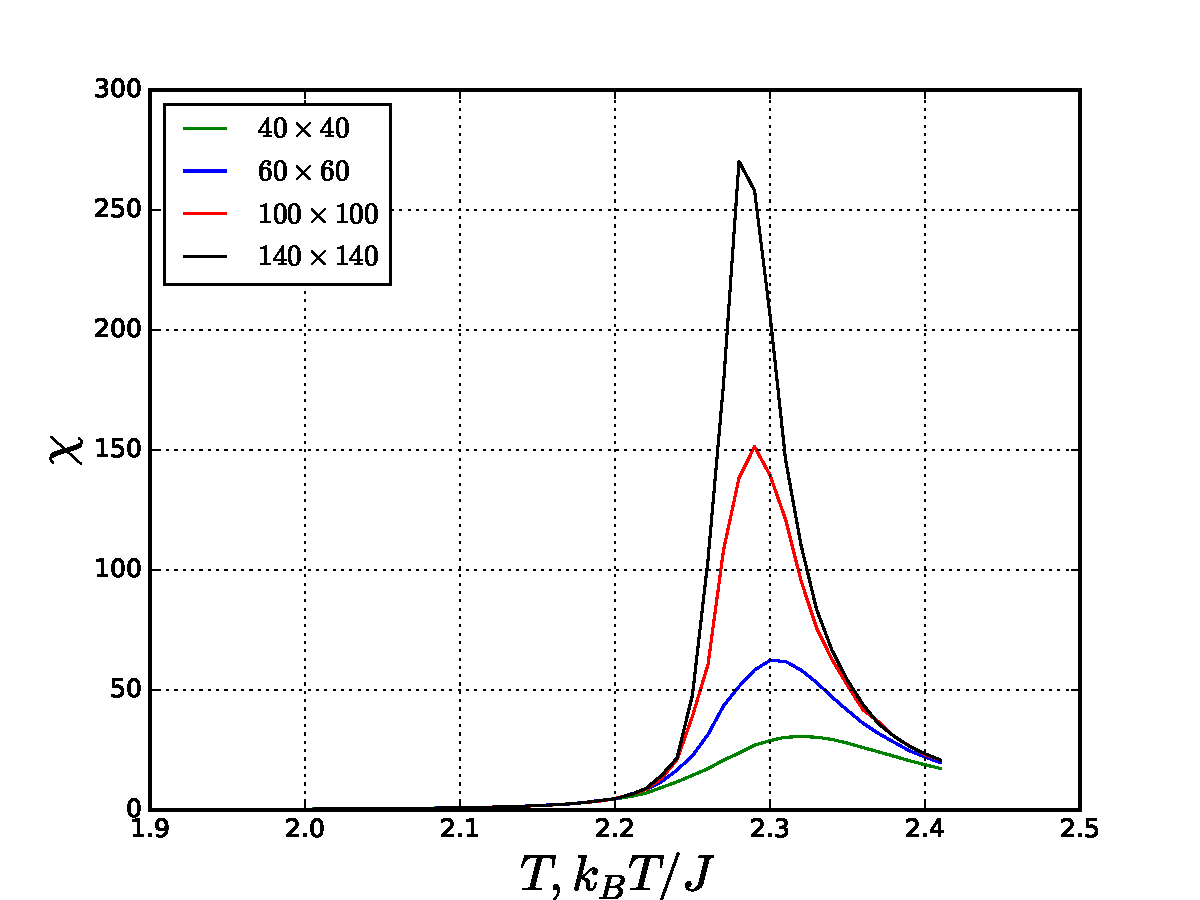
\includegraphics[width=1.0\linewidth]{phase_10_6_susceptability} 
    \caption{Susceptibility development over varying temperature } 
    \label{fig3:d} 
  \end{subfigure} 
  \caption{ Energy, magnetization, heat capacity and magnetic susceptibility development over varying temperature. Common diagrams for different lattice sizes ($40 \times 40$, $60 \times 60$, $100 \times 100$, $140 \times 140$). Number of MC samples is $10^6$. Temperature vary in range from 2.0 to 2.41, temperature step is 0.01. Temperature measured in $k_BT/J$ units.}
  \label{fig3} 
\end{figure}

\section{Conclusion and further research}\label{Conclusion}
In this project we used two dimensional Ising model to study the behavior of ferromagnetic material near the critical temperature. The material was modeled by square lattice. The Monte Carlo method was used together with Metropolis sampling rule to simulate the Markov processes. All obtain results are reasonable and agree with exact solutions.\\ 
This model have a large number of possibilities for further research. One may think about using triangular lattice instead of quadratic and then compare the results. Also it is possible to extend the model to tree dimensions without making a significant changes to the program. It is also possible to consider the situation with an external magnetic field present. Also, one can consider the long range interactions between spins (not only the nearest neighbors).\\
From the computational point of view it is possible to continue with parallelization. The one we implement here is the most simple one, however there a lot of possibilities to extend it and boost the computations.
\clearpage
\newpage
\begin{thebibliography}{one}

\bibitem{one} 
M. Plischke and B. Bergersen
\textit{Equilibrium Statistical Physics}. 
World Scientific, 2006.

\bibitem{two} 
Morten Hjorth-Jensen. 
\textit{Computational Physics
}. 
Lecture Notes Fall 2015, August 2015.



\bibitem{three} 
Charles Kittel
\textit{Introduction to Solid State Physics}. 
 Hoboken, NJ : Wiley,2005.

\bibitem{four}
E. Gabriel,  Graham E. Fagg and others.
\textit{OpenMPI: Goals, Concept, and Design of a Next Generation MPI Implementation}
Proceedings, 11th European PVM/MPI Users' Group Meeting, 2004


  
\end{thebibliography}
\end{document}
